\documentclass[10pt, a4paper]{amsart}

\usepackage[]{graphicx}
\usepackage[]{hyperref}
\usepackage[]{physics}
\usepackage[]{color,listings}
\usepackage[utf8]{inputenc}
\usepackage[toc,page]{appendix}

\definecolor{mygray}{gray}{0.6}

\lstset{
	frame = single,
	language = C++,
	showstringspaces = false,
	tabsize = 2,
	otherkeywords = {self},
	keywordstyle = \color{blue},
	identifierstyle=\color{blue},
 	stringstyle=\color{orange},
 	backgroundcolor=\color{mygray}
}

\title[Simulation of Solar System]{Simulation of Solar System Using Velocity Verlet Method \\
  \hrulefill\small{ FYS3150: Computational Physics }\hrulefill}

\author[Winther-Larsen \& Svalheim]{Sebastian G. Winther-Larsen \\ 
Trygve L. Svalheim \\
\href{https://github.com/gregwinther/FYS3150/}{\texttt{github.com/gregwinther}}}

\date{\today}

\begin{document}

\begin{titlepage}
\begin{abstract}
Two, three, multi. With Euler-Cromer and then Velocity Verlet
\end{abstract}
\maketitle
\tableofcontents
\end{titlepage}

\section{Introduction}

\section{Theory}

\subsection{Newtonian gravtiation}
When one studies the solar system and the way it moves, one inevitably needs to consider the gravity of the situation. The classical law of gravitation is given by Newton's law
\begin{equation}
\label{eq:newtoniangravity}
F_G = \frac{GM_1M_2}{r^2},
\end{equation} 
where $F_G$ is the gravitational force between to bodies, $G$\footnote{$G=6.67408 \times 10^{-11} m^3 kg^{-1} s{-2}$} is the gravitational constant, $M_1$ and $M_2$ are the masses of the two bodies and $r$ is the distance between them.

In three dimensions, by employing Newton's second law of motion, one will get the following componental equations for the acceleration due to gravitational pull on a particular body $i$.
\begin{equation}
\label{eq:componentalnewton}
\frac{d^2x}{dt^2} = \frac{F_{G,x}}{M_i}, \quad
\frac{d^2y}{dt^2} = \frac{F_{G,y}}{M_i}, \quad
\frac{d^2z}{dt^2} = \frac{F_{G,z}}{M_i},
\end{equation}
each of which can be integrated in order to find the position of the bodies at any given time and for a particular inital velocitiy and position. Moreover, a neat vectorial expression for the Newtonian gravity (equation \ref{eq:newtoniangravity}) in three dimensions is
\begin{equation}
\vb{F}_G = \frac{GM_1M_2}{r^3}\vb{r}
\end{equation}
where $\vb{r}$ gives the posistion of the body in a cartesian coordinate system.

\subsection{Relativity}

The theory of general relativity (GR), put forth by Albert Einstein in 1915, is the current description of gravity in modern physics. On curiosity of the solar system that cannot be explained is the perihelion precession of Mercury's orbit. For every Mercury year the perihelion of the planets orbit moves sligthly. The observed value of this effect is $43$ arc-seconds per century. Einstein showed himself that GR could explain this anomaly.

Closed elliptical orbits are a special feature of the factor ($1/r^2$) in Newton's law of gravitation. Any change to this factor will result in a change in the orbit. For a small such correction, each orbit will be almost the same, but as time progresses the orientation of the elliptical orbit will itself rotate. In this study we will not compute a space-time manifold in order to make this correction, but rather add a general relativistic error term to the Newtonian gravitational force (equation \ref{eq:newtoniangravity}.
\begin{equation}
\label{eq:relativenewton}
F_G = \frac{GM_{\odot}M_{Mercury}}{r^2}\left[1+\frac{3l^2}{r^2c^2} \right],
\end{equation}
where $M_{MERCURY}$ is the mass of Mercury, $r$ is the distance between Mercury and the Sun, $l=\abs{\vb{r}\times\vb{v}}$ is the orbital angular momentum per unit mass, and $c$ is the speed of light in vacuum.

\section{Units}
In order to make the system easy to work with and the calculations easier as well, a change of units is warranted. In this study we will therefore express the mass of any body as a fraction of solar masses, that is $M_{\odot} = 2\times10^{30}kg$. This means that the Earth\footnote{In SI-units, $M_{Earth}\approx6\times10^{24}kg$}, for instance will have a mass of $M_{Earth}= 3\times10^{-6}$.

Additionally, the units for distance will be astronmical units $AU$. This is the mean distance between the earth and the sun. For a simple system and a particular coordinate system with the sun at origin, the initial position for the Earth could simply be $\vb{r}_ {Earth}=(1,0,0)$.

The unit for time will be Earth years, $yr$. This means that velocity will be in units $AU/yr$.

Changing the variables will have consequences for the gravitationan constant $G$ and velocities $v$ as well. This can be deduced easily enough by picking a sample system consisting of the earth and the sun. Inserting in equation \ref{eq:newtoniangravity} gives
\begin{equation}
\label{eq:earthandsun}
F_G = \frac{GM_{\odot}M_{Earth}}{r^2}
\end{equation}
Furthermore, assuming the orbit of the earth is perfectly circular, will give the following relation
\begin{equation}
\label{eq:circularearth}
F_G = \frac{M_{Earth}v^2}{r}
\end{equation}
Combining equations \ref{eq:earthandsun} and \ref{eq:circularearth} yields the following
\begin{equation}
v^2r=gM_{\odot}=4\pi^2AU^3yr^{-2}
\end{equation}
Because the mass of the sun as a fraction of solar masses is $M_{\odot}=1$  and the distance between the earth and the sun is $r=1AU$ we land at
\begin{equation}
G=4\pi^2AU^3yr^{-2} \quad v_{Earth}=2\pi AUyr^{-1}
\end{equation}

\section{Algorithm and implementation}

\subsection{Object orientation}
Object orientation allows for more general code to be written and for easy reuse. Moreover, object orientation makes sense for humans, who tends to classify objects we see and interact with in everyday life. In this study we make use of all the advantages of object oriented programming by implementing several classes. A class diagram illustration of the program is included

The \lstinline|System| class contains all the information about the initial conditions of the system, which integration method should be used and also some helpful methods, like one that writes data to file.

The \lstinline|InitialCondition| superclass contains a method for setting up particles. Depending on what system one wants to model, we have implemented three subclasses of \lstinline|IntialCondition|: \lstinline|TwoBody|, \lstinline|ThreeBody| and \lstinline|MultiBody|. The name of these classes speek mostly for themselves.

The intersting objects, contained within the \lstinline|InitialCondition| subclasses are instances of the \lstinline|Particle| class. The class could have another name, like "planet" or "body" because instances of it will represent the largest bodies in the solar system; the sun and (eventually) all nine planets\footnote{Including Pluto for historical reasons.}.

\subsection{Euler-Cromer}

\subsection{Velocity Verlet}

\section{Data}

\section{Results}

\section{Discussion}

\section{Conclusion}

\pagebreak

\begin{appendix}

\section{Class Diagram}
\label{app:classdiagram}

\begin{figure}[ht]
	\centering
	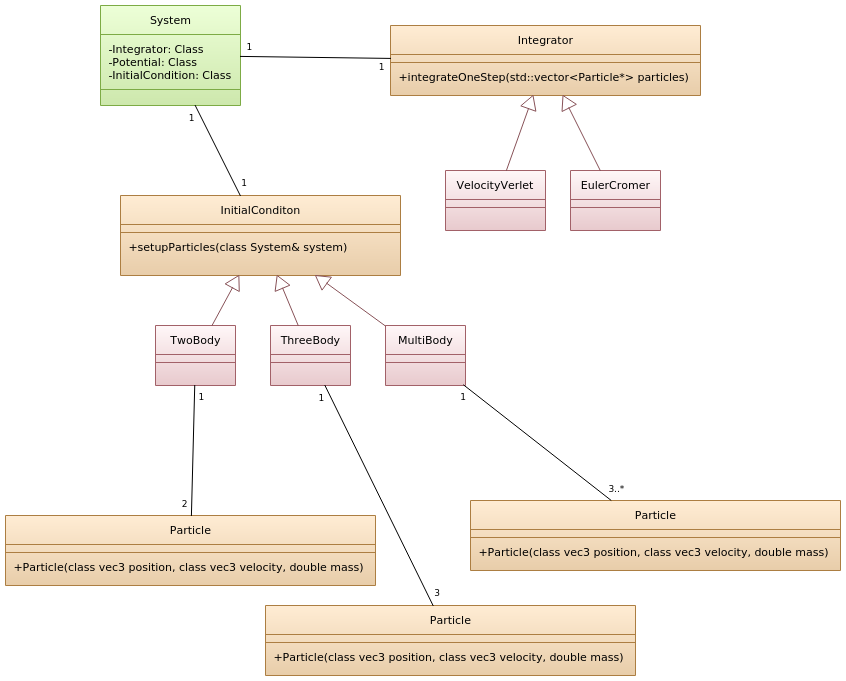
\includegraphics[width=0.9\textwidth]{../figures/classdiagram.png}
\end{figure}

\end{appendix}

\end{document}
